\documentclass[12pt]{article}

% Packages and formatting as in template
\usepackage{amsmath,amssymb,graphicx,booktabs,array,longtable,calc}
\usepackage{natbib}
\bibliographystyle{agsm}
\PassOptionsToPackage{hyphens}{url}
\usepackage[unicode]{hyperref}
\usepackage[dvipsnames,svgnames,x11names]{xcolor}
\usepackage{caption,subcaption,float}
\usepackage{microtype}
\usepackage{lmodern}
\usepackage{bookmark}

\setlength{\emergencystretch}{3em}
\setcounter{secnumdepth}{5}
\setlength{\parindent}{0pt}
\setlength{\parskip}{6pt plus 2pt minus 1pt}
\addtolength{\oddsidemargin}{-.5in}
\addtolength{\evensidemargin}{-.1in}
\addtolength{\textwidth}{1in}
\addtolength{\textheight}{1.7in}
\addtolength{\topmargin}{-1in}

\hypersetup{
  pdftitle={Faithful Spatial Attribution via Total-Variation Input Masking},
  pdfauthor={Robert Richardson},
  pdfkeywords={interpretable machine learning, spatial attribution, total variation, fused lasso, structured sparsity, CNN, El Nino},
  colorlinks=true,
  linkcolor={blue},
  citecolor={Blue},
  urlcolor={Blue}
}

\newcommand{\anon}{1} % Set to 0 for anonymized version

\begin{document}

\def\spacingset#1{\renewcommand{\baselinestretch}{#1}\small\normalsize}
\spacingset{1}

%%%%%%%%%%%%%%%%%%%%%%%%%%%%%%%%%%%%%%%%%%%%%%%%%%%%%%%%%%
% TITLE PAGE
%%%%%%%%%%%%%%%%%%%%%%%%%%%%%%%%%%%%%%%%%%%%%%%%%%%%%%%%%%

\if1\anon
{
  \title{\bf Faithful Spatial Attribution via Total-Variation Input Masking, with Application to El Ni\~no Forecasting}
  \author{Robert Richardson\thanks{
    Department of Statistics, Brigham Young University. }}
  \maketitle
} \fi

\if0\anon
{
  \bigskip \bigskip \bigskip
  \begin{center}
    {\LARGE\bf Title Goes Here}
  \end{center}
  \medskip
} \fi

\bigskip
\begin{abstract}
Attribution methods are widely used to explain the predictions of convolutional neural networks (CNNs) over spatial fields, but spatial dependence makes attribution ill-posed: when neighbouring inputs are highly correlated, predictive credit can be assigned almost arbitrarily among them, and post-hoc saliency maps become noisy and unstable. We study an in-model alternative in which a learnable input mask is trained jointly with the predictor and regularized by a \emph{structured-sparsity} penalty that combines an $\ell_1/\ell_2$-style sparsity term with a total-variation (TV) term encouraging spatial smoothness---the fused-lasso / Markov-random-field prior familiar from spatial statistics, applied here to a learned attribution map.

On synthetic data with known ground-truth signal and distractor regions, we show that (i) the TV penalty significantly improves the faithfulness of learned attribution and, applied as a modular add-on, improves not only our mask but also stochastic-gate baselines ($L_0$ and STG); and (ii) our TV+sparsity mask occupies a favourable point on the faithfulness--accuracy frontier, delivering faithful attribution without degrading---and slightly improving---predictive performance, whereas sparsity-only gates achieve marginally sharper localization only by collapsing the predictor. We apply the method to El Ni\~no prediction from sea-surface temperature: with the predictor selected honestly on a temporal validation split, the learned masks recover the known equatorial signal, agreeing with a lagged-correlation statistical reference, while coarse tiled masks remain competitive at a lower parameter count. We are explicit about limitations, including a failure mode in which sparsity-driven masks are captured by cheap spurious shortcuts.
\end{abstract}


\noindent%
{\it Keywords:} Interpretable machine learning; spatial attribution; structured sparsity; fused lasso; convolutional neural networks; sea surface temperature. % (Avoid duplicating words from title)

\vfill
\newpage
\spacingset{1.8}

%%%%%%%%%%%%%%%%%%%%%%%%%%%%%%%%%%%%%%%%%%%%%%%%%%%%%%%%%%
% MAIN SECTIONS
%%%%%%%%%%%%%%%%%%%%%%%%%%%%%%%%%%%%%%%%%%%%%%%%%%%%%%%%%%

\section{Introduction}\label{sec:intro}

Deep learning has become central to spatiotemporal environmental prediction---sea surface temperature (SST), atmospheric circulation, precipitation---where convolutional neural networks (CNNs) model high-dimensional, nonlinear fields with strong predictive skill \citep{Rasp2020WeatherBench,Bi2023PanguWeather,Pathak2022FourCastNet,Ham2019DLENSO}. In high-stakes geoscientific applications, however, predictions are only actionable if we can say \emph{where} on the field a model is drawing its information, and interpretability has become a research priority in its own right \citep{Toms2020PINN,Mamalakis2022Fidelity}. A central obstacle is that environmental inputs are strongly spatially dependent: neighbouring grid cells are highly correlated, so predictive credit can be distributed almost arbitrarily among them. As a result, gradient-based and perturbation-based attribution maps are typically diffuse, noisy, and unstable, and need not reflect the structure a domain scientist would call physical.

Two broad families of attribution exist. \emph{Post-hoc} methods explain an already-trained network: gradient saliency \citep{Simonyan2014Saliency}, integrated gradients \citep{Sundararajan2017IG}, Grad-CAM \citep{Selvaraju2017GradCAM}, and SHAP \citep{Lundberg2017SHAP} are widely used but can be unstable or manipulable and, being external to the model, need not reflect its internal feature use \citep{Adebayo2018Sanity,Ghorbani2019Fragile}. \emph{In-model} methods instead build attribution into training: gradient-regularized explanations \citep{Ross2017RRR,Ross2018GradReg}, class activation mapping \citep{Zhou2016CAM}, learned attention \citep{Hu2018SENet,Woo2018CBAM}, and---closest to our setting---learnable feature gates that select inputs jointly with the predictor, including $L_0$/hard-concrete gates \citep{Louizos2018L0}, stochastic gates \citep{Yamada2020STG}, and instance-wise selectors \citep{Chen2018L2X,Yoon2019INVASE}. These learned gates penalize \emph{sparsity} but treat input locations as exchangeable, with no notion of spatial structure---precisely what is needed when the inputs form a coherent field.

Our approach is in the in-model family: a learnable input mask, trained jointly with the predictor, that gates the input before prediction. Its distinguishing ingredient is a \emph{total-variation} (TV) penalty on the mask in addition to sparsity, so that the learned attribution is encouraged to be both compact and spatially contiguous. This pairing is exactly the structured-sparsity prior of the fused lasso \citep{Tibshirani2005FusedLasso} and total-variation denoising \citep{ROF1992} from spatial statistics, here imposed on a learned attribution map rather than on regression coefficients. The idea of combining TV with sparse attention has appeared inside per-token attention transforms for image captioning \citep{Martins2020TVMax}, and TV-regularized masks have been optimized \emph{post hoc}, one per image, against a frozen classifier \citep{Fong2017MeaningfulPerturbation,Dabkowski2017RealTime}; our contribution is to bring the smoothness prior to a single, globally-learned, in-model gate, to show on ground-truth data that it measurably improves faithfulness across gating mechanisms, and to apply it to environmental forecasting. We complement prior model-based interpretability such as prototype reasoning \citep{Chen2019ProtoPNet} and concept bottlenecks \citep{Koh2020CBM}.


Dropout, a widely used regularization technique in deep learning, operates by randomly masking neural units during training to prevent overfitting \citep{Hinton2012Dropout,Srivastava2014Dropout}. In CNNs, variants such as spatial dropout \citep{Tompson2015SpatialDropout,Wu2015DropoutCNN}, Cutout \citep{DeVries2017Cutout}, and random erasing \citep{Zhong2020RandomErasing} have been proposed to mask contiguous spatial regions and encourage robustness to occlusion.

Beyond random masking, partial convolution \citep{Liu2018PartialConv} and gated convolution \citep{Yu2019GatedConv} offer mechanisms for handling genuinely missing data or selectively attending to informative spatial locations. Gated mechanisms have also been used extensively in generative audio and language models \citep{Oord2016WaveNet,Dauphin2017GLU}, and more recently in environmental prediction tasks \citep{Zhang2024GatedRain}. Layer masking, proposed by \cite{Balasubramanian2023LayerMasking}, applies learned binary masks at intermediate layers to prevent distribution shifts caused by masked inputs. These methods collectively offer models structured decision processes and increased resilience to random noise. 

\subsection{Nonlinear Spatiotemporal Modeling in Environmental Science}

Traditional statistical models for environmental forecasting often rely on linear or quasi-linear dynamics, such as autoregressive models, Gaussian processes, and reduced-rank approximations \citep{banerjee2003hierarchical, cressie2015statistics}. However, nonlinearity has long been acknowledged as essential for capturing the dynamics of environmental systems \citep{wikle2010general}. Early work from the statistics community, including quadratic and bilinear extensions of state-space models, provided important foundations for nonlinear spatiotemporal modeling \citep{wikle2001spatiotemporal}.  These models predate the deep learning surge and remain central to understanding the dynamics of geophysical systems.

More recent statistical approaches, such as \cite{zammit2020deep} and \cite{wikle2023statistical}, integrate deep neural networks with hierarchical Bayesian frameworks to capture complex nonlinearities while preserving uncertainty quantification.

On the deep learning front, CNNs and ConvLSTMs \citep{Shi2015ConvLSTM} have been used to forecast meteorological and oceanographic variables, while benchmarks such as WeatherBench \citep{Rasp2020WeatherBench} have catalyzed comparative research in data-driven weather prediction. Subsequent models such as Pangu-Weather \citep{Bi2023PanguWeather} and FourCastNet \citep{Pathak2022FourCastNet} demonstrate that purely data-driven models can approach and even surpass numerical weather prediction (NWP) models at shorter lead times. These methods are increasingly being compared or combined with statistical spatiotemporal approaches, such as those proposed by \cite{zammit2020deep}, to evaluate tradeoffs between interpretability, uncertainty quantification, and predictive power.


\section{Methods}\label{sec:methods}

We propose a model-integrated attribution framework for convolutional neural networks (CNNs) based on learnable input masking. The goal of our approach is to embed spatial interpretability directly into the predictive model, such that saliency maps arise as a natural product of training rather than requiring post hoc analysis. This is achieved by integrating a learnable masking module into the architecture and regularizing it to produce sparse and spatially coherent masks.

\subsection{Model Architecture}

Let \( x \in \mathbb{R}^{H \times W} \) denote an input spatial feature map. The model learns a real-valued spatial mask \( m \in [0, 1]^{H \times W} \), which is applied elementwise to the input via Hadamard product, yielding a masked input \( \tilde{x} = x \odot m \). This masked input is passed to a convolutional neural network \( f_\theta(\cdot) \), yielding prediction \( \hat{y} = f_\theta(\tilde{x}) \). The mask \( m \) is itself a function of the input, computed by a gating mechanism \( g_\phi(x) \), where \( \phi \) denotes the parameters of the mask module.

To construct the mask, each spatial location \( k \) is associated with a learnable importance score \( z_k^{(m)} \in \mathbb{R} \). These scores are passed through a temperature-controlled sigmoid activation:

\[
m_k = \sigma\left( \frac{z_k^{(m)}}{\tau} \right),
\]

where \( \sigma(\cdot) \) denotes the standard sigmoid function and \( \tau > 0 \) is a temperature parameter controlling the sharpness of the activation. The masked input is then given by

\[
\tilde{x}_k = m_k \cdot x_k,
\]

where each pixel is modulated by its corresponding mask value. This mechanism allows the model to dynamically suppress or retain information from each spatial location, based on its learned relevance to the prediction task. The mask acts as a differentiable gating layer, encouraging the model to focus on a sparse and interpretable subset of input regions.



\subsection{Loss Function and Regularization}

Training proceeds by minimizing a composite loss function that balances predictive performance with interpretability. The loss is defined as:

\begin{equation}
\mathcal{L} = \mathrm{BCE}(\hat{y}, y)
+ \lambda_{\text{sp}} \cdot \frac{1}{K} \sum_{k} |m_k|^\gamma
+ \lambda_{\text{TV}} \cdot \frac{1}{|\mathcal{N}|} \sum_{(i,j)\in\mathcal{N}} |m_i - m_j|^\gamma
\label{eq:loss1}
\end{equation}

\begin{itemize}
    \item \( \mathrm{BCE}(\hat{y}, y) \) is the binary cross-entropy loss between the predicted logits \( \hat{y} \) and the true label \( y \).
    \item The sparsity penalty (weighted by \( \lambda_{\text{sp}} \)) encourages the mask to be sparse, limiting the number of significant spatial locations.
    \item The total variation term (weighted by \( \lambda_{\text{TV}} \)) promotes spatial smoothness in the mask by penalizing the absolute differences between neighboring pixel values. Here, \( \mathcal{N} \) denotes the set of adjacent pixel pairs.
\end{itemize}

All regularization terms are normalized by the number of spatial units (or pairs) to ensure consistent behavior across different input resolutions. The exponent parameter \( \gamma \in \{1, 2\} \) controls the form of the penalization. When \( \gamma = 1 \), the regularization promotes sparsity in the style of an \( \ell_1 \)-norm penalty, while \( \gamma = 2 \) corresponds to an \( \ell_2 \)-style penalty that encourages small but diffuse activations. In our experiments, both values produced qualitatively similar saliency masks, with \( \gamma = 2 \) typically yielding smoother and lower-magnitude mask activations. This choice offers a tunable trade-off between promoting sharp selectivity and preserving gradient stability during optimization.

\paragraph{A structured-sparsity prior.}
The two penalties in \eqref{eq:loss1} together impose a \emph{structured-sparsity} prior on the mask: the sparsity term limits the number of active locations, while the total-variation term couples neighbouring locations so that active regions are spatially contiguous rather than scattered. This is precisely the prior underlying the fused lasso \citep{Tibshirani2005FusedLasso} and total-variation denoising \citep{ROF1992}, and is equivalent to a maximum-a-posteriori estimate under a Laplacian Markov-random-field smoothness prior combined with a sparsity-inducing marginal---a combination long used for spatial regularization in statistics. What is new here is the \emph{target} of the prior: rather than regularizing regression coefficients or a post-hoc per-image perturbation mask \citep{Fong2017MeaningfulPerturbation,Dabkowski2017RealTime}, or a per-token attention transform \citep{Martins2020TVMax}, we regularize a single, globally-learned, in-model attribution gate that is trained jointly with the predictor. In Section~\ref{sec:sim} we show on ground-truth data that the smoothness term measurably improves attribution faithfulness, and that this benefit is not specific to our gate but transfers to other learned gates ($L_0$, STG) as a modular add-on.


\subsection{Temperature Annealing}

To encourage discrete, interpretable mask behavior, we apply a sigmoid activation with a temperature parameter \( \tau > 0 \) that is annealed over the course of training. The temperature controls the sharpness of the sigmoid response: larger values of \( \tau \) produce smoother, more graded activations, while smaller values yield sharper, near-binary outputs. 

As a general rule, we initialize \( \tau > 1 \) to allow for soft, flexible mask values during early training, and gradually reduce \( \tau \) to a value below 1 to promote sharper, more selective gating. For example, we linearly anneal \( \tau \) from 2.0 to 0.5 across training epochs. This schedule encourages exploration in the early stages of learning and supports convergence toward sparse, high-confidence mask values as training progresses.

Critically, this temperature annealing also helps avoid degenerate solutions where all mask values saturate toward 0 or 1 simultaneously. By maintaining intermediate \( \tau \) values during training, the model preserves meaningful gradients and can differentiate between relevant and irrelevant input regions.


\subsection{Training Procedure}

The full model, including both the predictive network and the masking mechanism, is trained end-to-end using optimization methodology such as stochastic gradient descent with the Adam optimizer. All components are fully differentiable: the mask values \( m_k \) are smooth functions of underlying latent variables \( z_k^{(m)} \), which enables gradients to flow from the loss through the masked input and back to both the mask parameters \( \phi \) and the network parameters \( \theta \) during backpropagation.

Specifically, the gradient of the loss with respect to each importance score \( z_k^{(m)} \) is computed via the chain rule using the derivative of the sigmoid activation:
\[
\frac{\partial \mathcal{L}}{\partial z_k^{(m)}} = \frac{\partial \mathcal{L}}{\partial m_k} \cdot \sigma'\left( \frac{z_k^{(m)}}{\tau} \right) \cdot \frac{1}{\tau},
\]
where \( \sigma'(z) = \sigma(z)(1 - \sigma(z)) \) is the derivative of the sigmoid function. This enables efficient gradient-based optimization without the need for numerical differentiation or reinforcement-style gradient estimators.

\subsection{Computational Considerations}

The addition of a learnable input mask introduces extra computational cost during training, with the extent of this overhead depending strongly on the spatial resolution of the input rather than the number of training examples. The gating mechanism requires learning a set of latent importance scores \( \{ z_k^{(m)} \} \), which are passed through a temperature-controlled sigmoid and applied elementwise to the input. Although this adds negligible memory or compute for small spatial domains, the cost becomes more pronounced as the spatial resolution increases.

In particular, the total variation penalty—which computes finite differences between adjacent spatial elements—scales with the number of spatial locations and must be evaluated and backpropagated at every iteration. While this operation is vectorizable and parallelizable, it becomes a computational bottleneck for high-resolution grids (e.g., \(64 \times 64\) or larger). In contrast, increasing the number of training samples (batch size or dataset size) has minimal impact on this cost, as the masking operation is applied independently across batches.

To address this scalability issue, we also consider a tiled version of the mask. The input domain is divided into \( K \) non-overlapping tiles (e.g., \(10 \times 10\)), and each tile \( k \in \{1, \dots, K\} \) is assigned a learnable importance score \( z_k^{(m)} \). These scores are transformed into mask values via a temperature-controlled sigmoid:
\(
m_{G_k} = \sigma\left( z_k^{(m)}/\tau \right),
\)
and the masked input is constructed by broadcasting the tile-level gate to all pixels in the tile:
\(
\tilde{x}_{i,j} = m_{G_k} \cdot x_{i,j},
\)
where \( G_k \) denotes the tile index to which location \( (i, j) \) belongs.

This tiling strategy dramatically reduces the number of learned mask parameters—from one per pixel to one per tile—and eliminates the need to compute fine-grained total variation penalties. As a result, training time and memory usage are significantly reduced for high-resolution spatial data. Although this approach produces coarser attribution maps, the loss in granularity can be offset by improved semantic clarity: in many real-world forecasting settings, highlighting important regions (e.g., ocean basins, pressure zones) may be more interpretable and actionable than identifying individual pixels.

Despite the increased training cost, our approach remains far more efficient than perturbation-based attribution techniques such as SHAP or occlusion, which require repeated forward passes for each input. Once trained, both the per-pixel and tiled mask variants incur negligible overhead at inference time, producing predictions and saliency maps in a single forward pass.


\section{Simulation Study: Faithful Attribution under Known Ground Truth}\label{sec:sim}

Because faithfulness cannot be measured directly on real data, we evaluate it on synthetic
data with a known predictive structure, following the now-standard practice of benchmarking
explanations against ground truth in the geosciences \citep{Mamalakis2022Fidelity}. We ask three
questions: (i) does the total-variation penalty improve the faithfulness of a learned mask;
(ii) is any such benefit specific to our gate, or does it transfer to other in-model gates; and
(iii) how does our mask compare to both post-hoc and learned-gate baselines on faithfulness
\emph{and} predictive performance.

\subsection{Data and metrics}
Each image is $24\times48$ with i.i.d.\ Gaussian background noise
$x_{i,j}\sim\mathcal N(0,0.5^2)$, and the dataset has $N=500$ samples. Two circular
\emph{signal} regions (A at $(10,15)$ and B at $(14,30)$, radius 4) and two \emph{distractor}
regions (radius 3) each receive a per-sample $\mathcal N(0,1)$ coefficient. The binary label is
an XOR over the mean intensities of A and B---the label is 1 iff exactly one exceeds 0.5---so
the task is nonlinear (requiring a CNN) and the distractors are, by construction, uninformative.
We score each method's $H\times W$ importance map against the known regions by
Intersection-over-Union (IoU, using the top-10\% most salient pixels) and by attribution mass
(the fraction of total map mass inside a region). Higher signal overlap and lower distractor
overlap are better.

\subsection{Methods compared}
We compare three families on a shared two-convolution backbone. \emph{Post-hoc} attributions are
computed on an ungated CNN---gradient saliency \citep{Simonyan2014Saliency}, integrated
gradients \citep{Sundararajan2017IG}, Grad-CAM \citep{Selvaraju2017GradCAM}, and gradient
SHAP \citep{Lundberg2017SHAP}, all via Captum \citep{Kokhlikyan2020Captum}. \emph{Learned
in-model gates} are trained jointly with the predictor: an $L_0$ hard-concrete gate
\citep{Louizos2018L0}, a stochastic gate (STG) \citep{Yamada2020STG}, and a CBAM-style spatial
attention gate \citep{Woo2018CBAM}. \emph{Our mask} is the temperature-annealed sigmoid gate of
Section~\ref{sec:methods} with sparsity and TV penalties, reported both with and without the TV
term (the within-method ablation). All results are averaged over 15 random seeds; comparisons use
the paired Wilcoxon signed-rank test.

\begin{figure}[htbp]
  \centering
  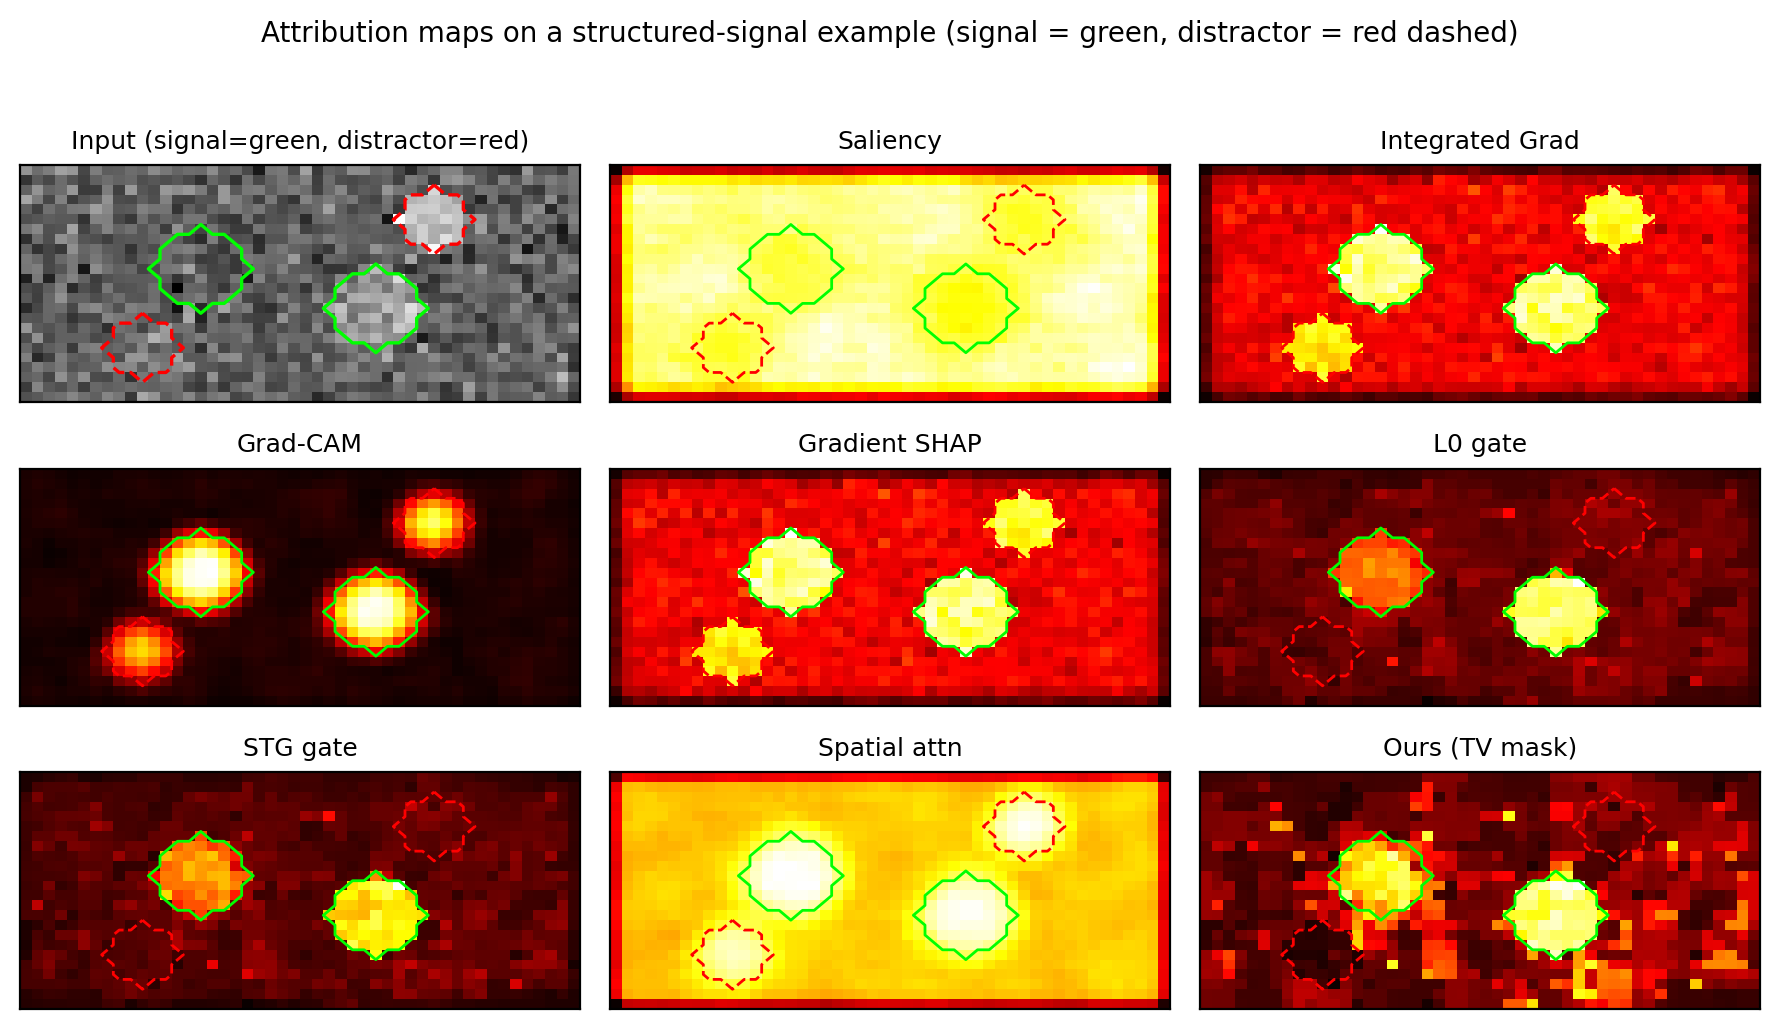
\includegraphics[width=0.95\textwidth]{sim1_attributions.png}
  \caption{Attribution maps from each method on a representative test image. Signal regions are
    outlined in green, distractors in red dashed. Post-hoc gradient maps are diffuse and leak onto
    the distractors; the learned gates concentrate on the signal, and our TV mask produces a
    compact, contiguous attribution over the true regions.}
  \label{fig:sim-attrib}
\end{figure}

\subsection{Total variation improves faithfulness}
Table~\ref{tab:sim} and Figure~\ref{fig:sim-bar} report faithfulness and predictive performance.
Removing the TV term from our mask reduces signal IoU from $0.747$ to $0.453$ (paired Wilcoxon
$p=10^{-4}$): without spatial coupling the mask selects a sparse, incomplete subset of the signal,
whereas the TV term fills in the contiguous predictive region. Every learned gate suppresses the
distractors strongly (IoU $\le 0.01$), while post-hoc gradient maps leak substantially onto them
(IoU $0.15$--$0.22$).

\begin{table}[htbp]
\centering
\caption{Attribution faithfulness and predictive performance on the structured-signal simulation
  (mean over 15 seeds). Signal IoU: higher is better; distractor IoU: lower is better. The last
  column is the paired Wilcoxon $p$-value for signal IoU against Ours (TV).}
\label{tab:sim}
\begin{tabular}{lccccc}
\toprule
\textbf{Method} & \textbf{Signal IoU} & \textbf{Distr.\ IoU} & \textbf{Acc} & \textbf{F1} & \textbf{$p$ vs ours} \\
\midrule
Saliency             & 0.454 & 0.215 & 0.673 & 0.539 & $10^{-4}$ \\
Integrated gradients & 0.786 & 0.146 & 0.673 & 0.539 & 0.17 \\
Grad-CAM             & 0.669 & 0.210 & 0.673 & 0.539 & 0.009 \\
Gradient SHAP        & 0.785 & 0.146 & 0.673 & 0.539 & 0.14 \\
$L_0$ gate           & 0.836 & 0.002 & 0.626 & 0.419 & 0.002 \\
STG gate             & 0.840 & 0.003 & 0.579 & 0.276 & 0.002 \\
Spatial attention    & 0.610 & 0.199 & 0.675 & 0.547 & 0.003 \\
Ours (no TV)         & 0.453 & 0.000 & 0.723 & 0.631 & $10^{-4}$ \\
\textbf{Ours (TV)}   & 0.747 & 0.000 & 0.716 & 0.620 & --- \\
\bottomrule
\end{tabular}
\end{table}

\begin{figure}[htbp]
  \centering
  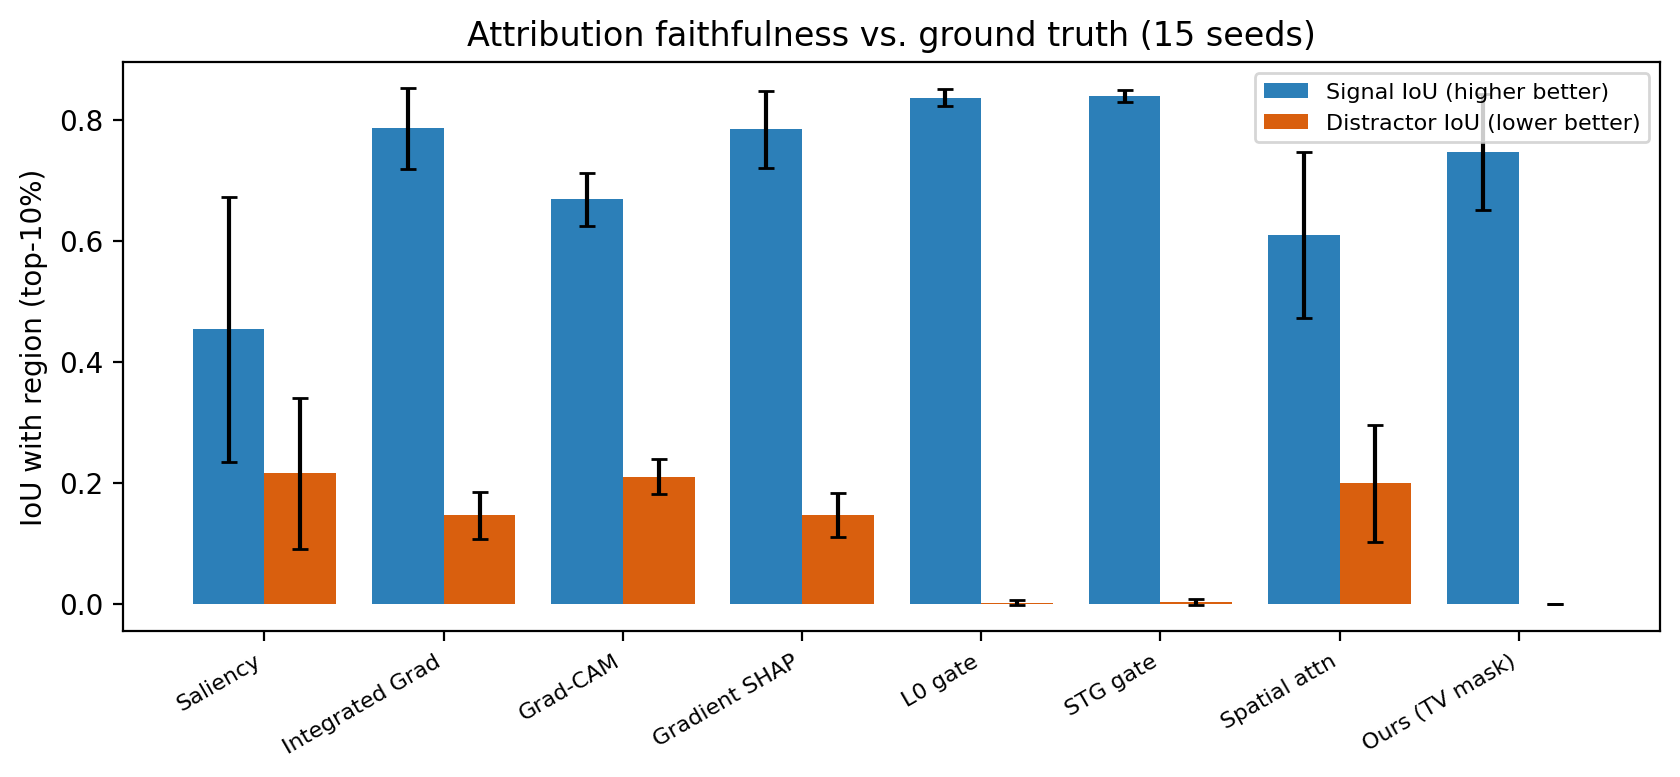
\includegraphics[width=0.85\textwidth]{sim1_faithfulness.png}
  \caption{Signal- and distractor-region IoU per method (mean $\pm$ SD over 15 seeds). Learned
    gates suppress distractors; the TV term lifts our mask's signal overlap without inflating
    distractor overlap.}
  \label{fig:sim-bar}
\end{figure}

\subsection{The smoothness prior transfers across gates}
Because total variation regularizes any differentiable spatial map, it can be added to other
in-model gates as a modular term. We swept the sparsity weight for the $L_0$, STG, and our own
gate, each with TV off and on, and measured the change in signal IoU
(Figure~\ref{fig:sim-modular}). Adding TV significantly improves the $L_0$ and STG gates, provided
they are not already saturated: at moderate sparsity the gain in signal IoU is $+0.07$ for $L_0$
(paired Wilcoxon $p=0.012$) and $+0.13$ for STG ($p=0.008$); at very high sparsity both gates
already localize tightly and TV adds little. Strikingly, all three gates collapse onto a common
curve: the IoU gain from TV is governed by how well the base gate localizes \emph{without} it---
largest when the base gate is poor, shrinking to zero at the ceiling---and not by which gating
mechanism is used. The smoothness prior therefore behaves as a general, modular improvement to
learned spatial attribution rather than a quirk of our particular gate. We fixed the TV weight
across methods rather than tuning it per gate; a per-method sensitivity analysis is left to the
supplement.

\begin{figure}[htbp]
  \centering
  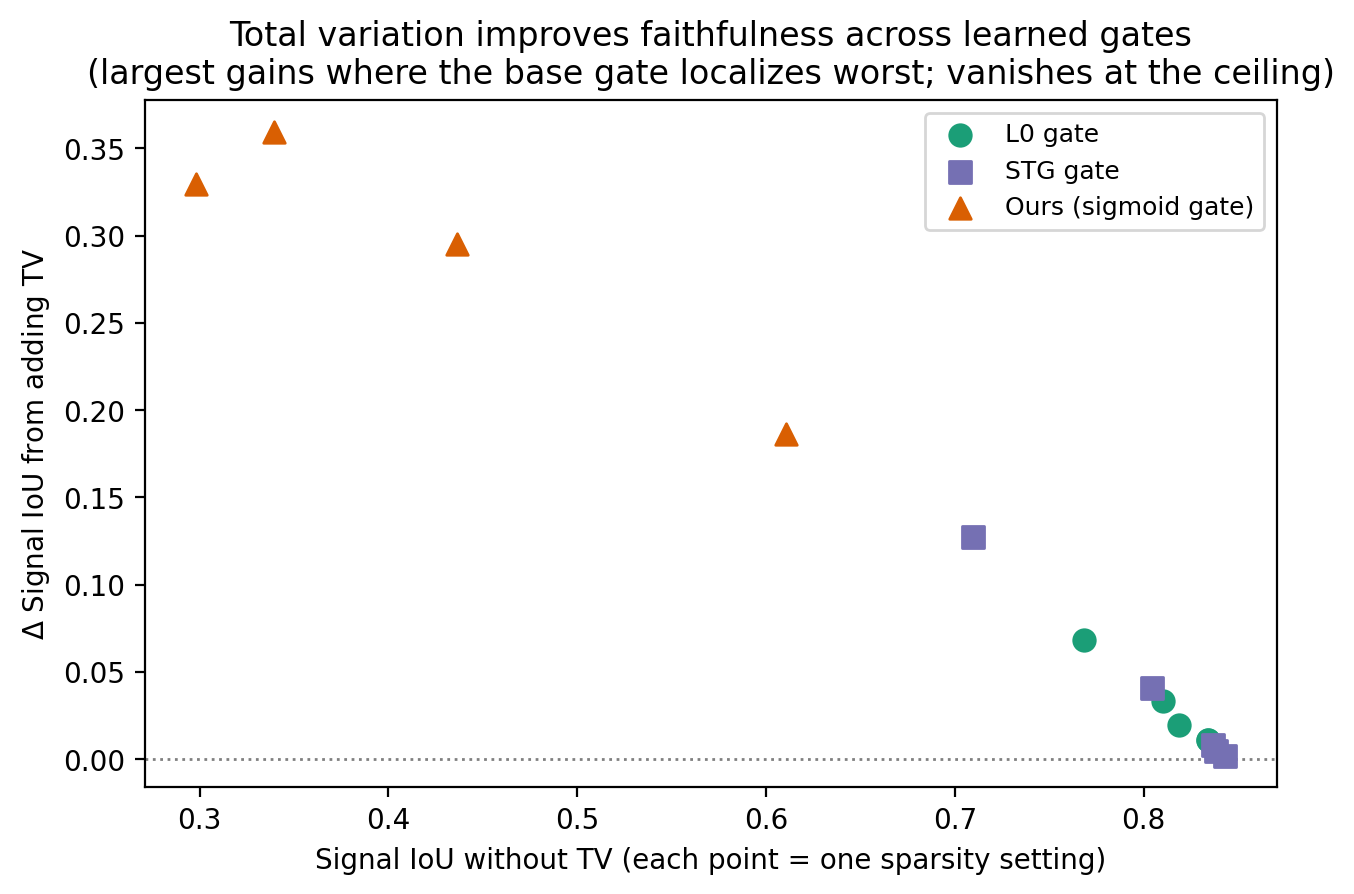
\includegraphics[width=0.72\textwidth]{sim1_modular_tv.png}
  \caption{The total-variation penalty as a modular faithfulness prior. Each point is one
    sparsity setting of one gate; the vertical axis is the change in signal IoU from adding TV.
    Every point lies at or above zero (TV never hurts faithfulness), and the three gates ($L_0$,
    STG, and ours) fall on a common curve: the gain is largest where the base gate localizes worst
    and vanishes once it already saturates the IoU ceiling.}
  \label{fig:sim-modular}
\end{figure}

\subsection{A faithfulness--accuracy frontier}
Sweeping the sparsity weight also traces out a frontier between localization and prediction
(Figure~\ref{fig:sim-frontier}). The sparsity-only gates ($L_0$, STG) reach the highest signal
IoU ($\approx 0.84$), but only at low predictive performance: their best attainable F1 is
$\approx 0.46$--$0.48$, at or below the ungated baseline, because hard sparsification discards
information the predictor needs. Our TV+sparsity mask instead reaches F1 $\approx 0.63$---
significantly higher than either gate (paired Wilcoxon $p=0.002$) and above the ungated
baseline---while still attaining signal IoU up to $0.80$ (a small but significant deficit of
$0.045$ relative to the sparsity-only ceiling, $p=0.043$). For an attribution mechanism this is
the more useful operating point: a faithful explanation that does not require degrading the model
it explains. The soft, smooth mask attenuates rather than deletes inputs, which both preserves
predictive signal and---through the TV prior---keeps the attribution spatially coherent.

\begin{figure}[htbp]
  \centering
  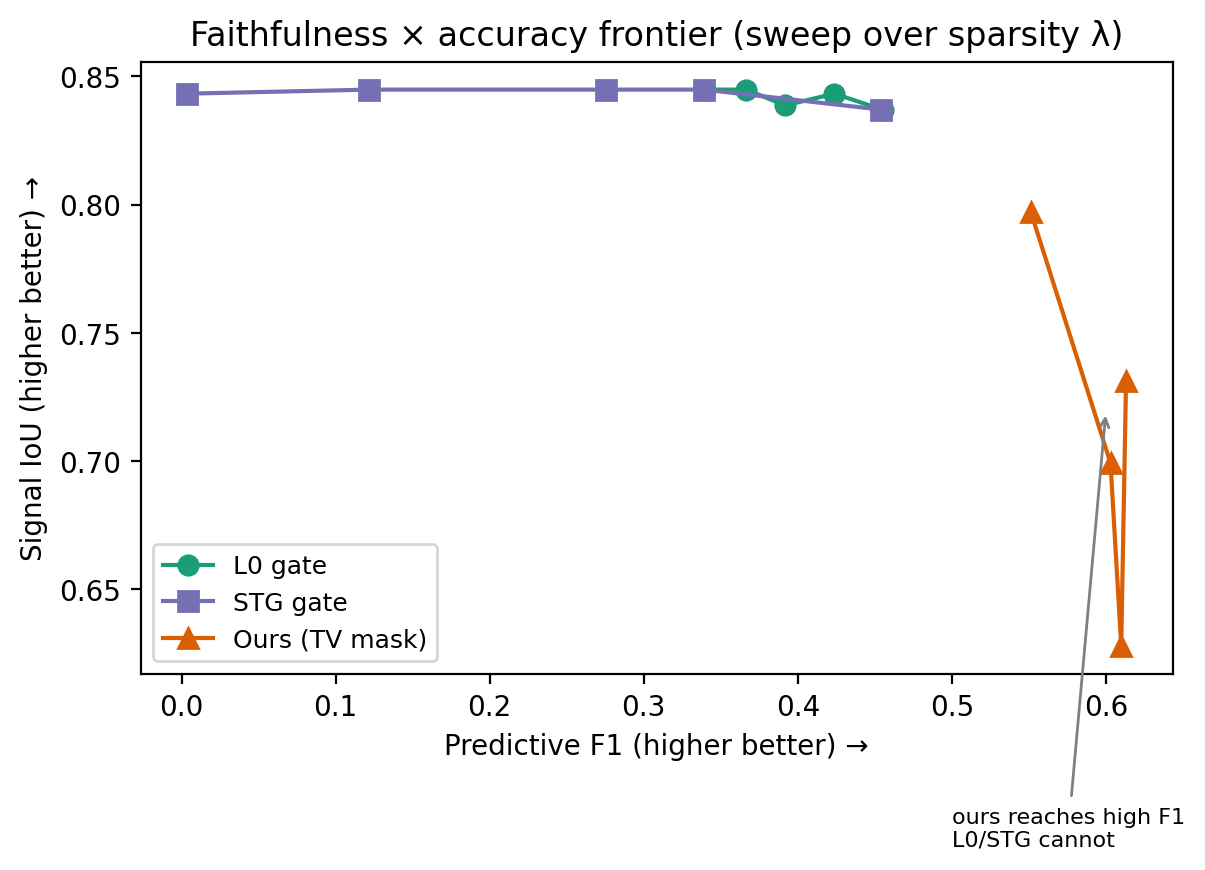
\includegraphics[width=0.75\textwidth]{sim1_frontier.png}
  \caption{Faithfulness--accuracy frontier as the sparsity weight is varied (TV on). Sparsity-only
    gates occupy the high-IoU, low-F1 region; our TV mask occupies the high-F1 region they cannot
    reach, at strong signal IoU and zero distractor overlap.}
  \label{fig:sim-frontier}
\end{figure}

\subsection{Limitation: capture by spurious shortcuts}\label{sec:sim-limitation}
The sparsity penalty rewards concentrating mask mass on the \emph{cheapest} predictive region.
When a non-causal feature is cheaply predictive---for instance a single region whose sign is
correlated with the label---the mask can be drawn onto it in preference to a more distributed
causal signal. In a variant in which a spurious region encoded a noisily-flipped copy of the
label, our mask concentrated on the spurious region (signal IoU $0.06$) while post-hoc integrated
gradients still recovered the causal regions (IoU $0.71$). We therefore do \emph{not} claim
robustness to spurious correlation; characterizing when sparsity-driven masking resists versus is
captured by shortcut features is important future work.

\section{Application: Predicting El Ni\~no from Sea-Surface Temperature}\label{sec:enso}

We now apply the masking framework to a real spatiotemporal forecasting problem with strong
spatial dependence---predicting El Ni\~no from sea-surface temperature (SST). Deep networks
forecast the El Ni\~no--Southern Oscillation with useful skill \citep{Ham2019DLENSO}, and
interpreting \emph{where} on the Pacific they draw that skill is of direct scientific interest
\citep{Toms2020PINN}. SST is also an ideal stress test for the attribution-under-dependence
problem: the equatorial Pacific is highly autocorrelated, so predictive credit is intrinsically
hard to localize. We ask two questions: does input gating preserve predictive skill, and do the
learned masks agree with a principled statistical attribution?

\subsection{Data and set-up}
We use monthly SST anomalies over the tropical Pacific ($15^\circ$S--$15^\circ$N,
$170^\circ$E--$100^\circ$W), de-seasonalized against the monthly climatology and down-sampled to a
$30\times90$ grid. The binary label is an El Ni\~no event---the Ni\~no-3.4 anomaly
($5^\circ$S--$5^\circ$N, $190^\circ$--$240^\circ$E) exceeding $0.5^\circ$C---at a lead of $k$
months; the event rate is $\approx 27\%$. We report leads $k=3$ and $k=6$.

We guard against two sources of optimism. First, SST is strongly autocorrelated in time, so a
random train/validation split leaks; we use a strictly \emph{temporal} division of the months
into train (earliest $60\%$), validation ($60$--$80\%$), and a held-out test block (last $20\%$).
Second, rather than fixing an architecture by hand---and risking the over-parameterization typical
of inherited specifications---we \emph{select} the backbone on the validation block. We compared
five candidate CNNs spanning $1.3$k--$288$k parameters (including the five-layer DeepCNN of the
prior specification) by the validation AUROC of the ungated predictor
(Table~\ref{tab:enso-select}). The large DeepCNN---roughly $700$ parameters per training month---
generalizes \emph{worst}; the selected model is a compact CNN with $\approx\!5$k parameters (two
$3\times3$ convolutions with $2\times2$ pooling, batch normalization and ReLU, global average
pooling, and a linear head). \emph{All final numbers below are reported on the untouched test
block}, which played no part in selection.

\begin{table}[htbp]
\centering
\caption{Architecture selection by validation AUROC (mean over leads 3 and 6, ungated baseline).
  The inherited DeepCNN is the most over-parameterized and generalizes worst.}
\label{tab:enso-select}
\begin{tabular}{lcc}
\toprule
\textbf{Backbone} & \textbf{Parameters} & \textbf{Validation AUROC} \\
\midrule
Compact CNN (selected) & 4{,}929   & \textbf{0.890} \\
Medium CNN             & 25{,}633  & 0.884 \\
Medium CNN (GELU)      & 25{,}633  & 0.881 \\
Tiny CNN               & 1{,}313   & 0.880 \\
DeepCNN (prior spec)   & 288{,}385 & 0.874 \\
\bottomrule
\end{tabular}
\end{table}

Given the selected backbone we train the ungated baseline and the pixel, $2\times2$, and
$4\times4$ gates of Section~\ref{sec:methods} with sparsity ($\lambda_{\mathrm{sp}}=10^{-2}$) and
total-variation ($\lambda_{\mathrm{TV}}=0.2$) penalties and temperature annealing
($\tau:2.0\!\to\!0.01$), using Adam with multiplicative input dropout and early stopping on the
validation AUROC. The TV weight was chosen by a small sweep over $\{0.01,0.05,0.2,0.5\}$ that
maximized mask agreement with the statistical reference (below) at unchanged AUROC. All numbers
are means over three seeds.

\subsection{Predictive performance}
Table~\ref{tab:enso} reports test-block performance. We emphasize AUROC, a threshold-free ranking
metric, because the $0.5$ decision threshold is poorly calibrated on a held-out \emph{future}
block whose event frequency differs from the training period---the threshold-dependent accuracy
and F1 degrade accordingly and should be read with caution. At lead 3 the model ranks events well
(AUROC $\approx 0.82$); at lead 6 skill is marginal (AUROC $\approx 0.62$): six-month ENSO
prediction from SST alone, evaluated strictly out-of-time, is genuinely difficult. The key point
for our purposes is that \emph{gating does not degrade prediction}---gated and ungated models are
within error at both leads---so, as in the simulations, the mask buys interpretability essentially
for free.

\begin{table}[htbp]
\centering
\caption{El Ni\~no prediction on the held-out \emph{test} block (mean over 3 seeds), with the
  selected compact backbone. AUROC is the reliable metric here; accuracy and F1 are depressed by
  threshold miscalibration under temporal distribution shift. ``Agree'' is the Pearson correlation
  between the seed-averaged mask and the magnitude of the lagged-correlation reference
  (Section~\ref{sec:enso-ref}).}
\label{tab:enso}
\begin{tabular}{llcccc}
\toprule
\textbf{Lead} & \textbf{Gate} & \textbf{AUROC} & \textbf{Accuracy} & \textbf{F1} & \textbf{Agree} \\
\midrule
3 mo & None            & 0.822 & $0.55\pm0.21$ & 0.45 & --- \\
3 mo & Pixel           & 0.826 & $0.57\pm0.22$ & 0.35 & $\mathbf{0.63}$ \\
3 mo & Tiled 2$\times$2 & 0.826 & $0.57\pm0.22$ & 0.34 & $0.57$ \\
3 mo & Tiled 4$\times$4 & 0.826 & $0.57\pm0.22$ & 0.35 & $0.62$ \\
\midrule
6 mo & None            & 0.622 & $0.70\pm0.03$ & 0.10 & --- \\
6 mo & Pixel           & 0.621 & $0.72\pm0.02$ & 0.05 & $0.50$ \\
6 mo & Tiled 2$\times$2 & 0.618 & $0.72\pm0.02$ & 0.05 & $0.43$ \\
6 mo & Tiled 4$\times$4 & 0.619 & $0.70\pm0.03$ & 0.10 & $0.26$ \\
\bottomrule
\end{tabular}
\end{table}

\subsection{A statistical reference for attribution}\label{sec:enso-ref}
Real SST has no ground-truth attribution, so we validate the masks by \emph{convergent validity}
against a principled statistical reference: the per-cell lagged point-biserial correlation between
the SST anomaly and the future label (Figure~\ref{fig:enso-ref}, left). This map shows the
expected structure---a tight equatorial warm-tongue band at lead 3 that broadens into the
sub-tropics by lead 6. We also fit a fused-lasso logistic regression ($\ell_1$ + TV penalties on
the per-cell coefficients), the linear statistical sibling of our mask. It is, however, hampered
by collinearity: with $p \gg n$ and near-indistinguishable neighbouring equatorial cells, the
coefficients are unstable even under strong regularization (Figure~\ref{fig:enso-ref}, right)---
itself a vivid illustration of the attribution problem. We therefore use the robust univariate
correlation map as the reference.

\begin{figure}[htbp]
  \centering
  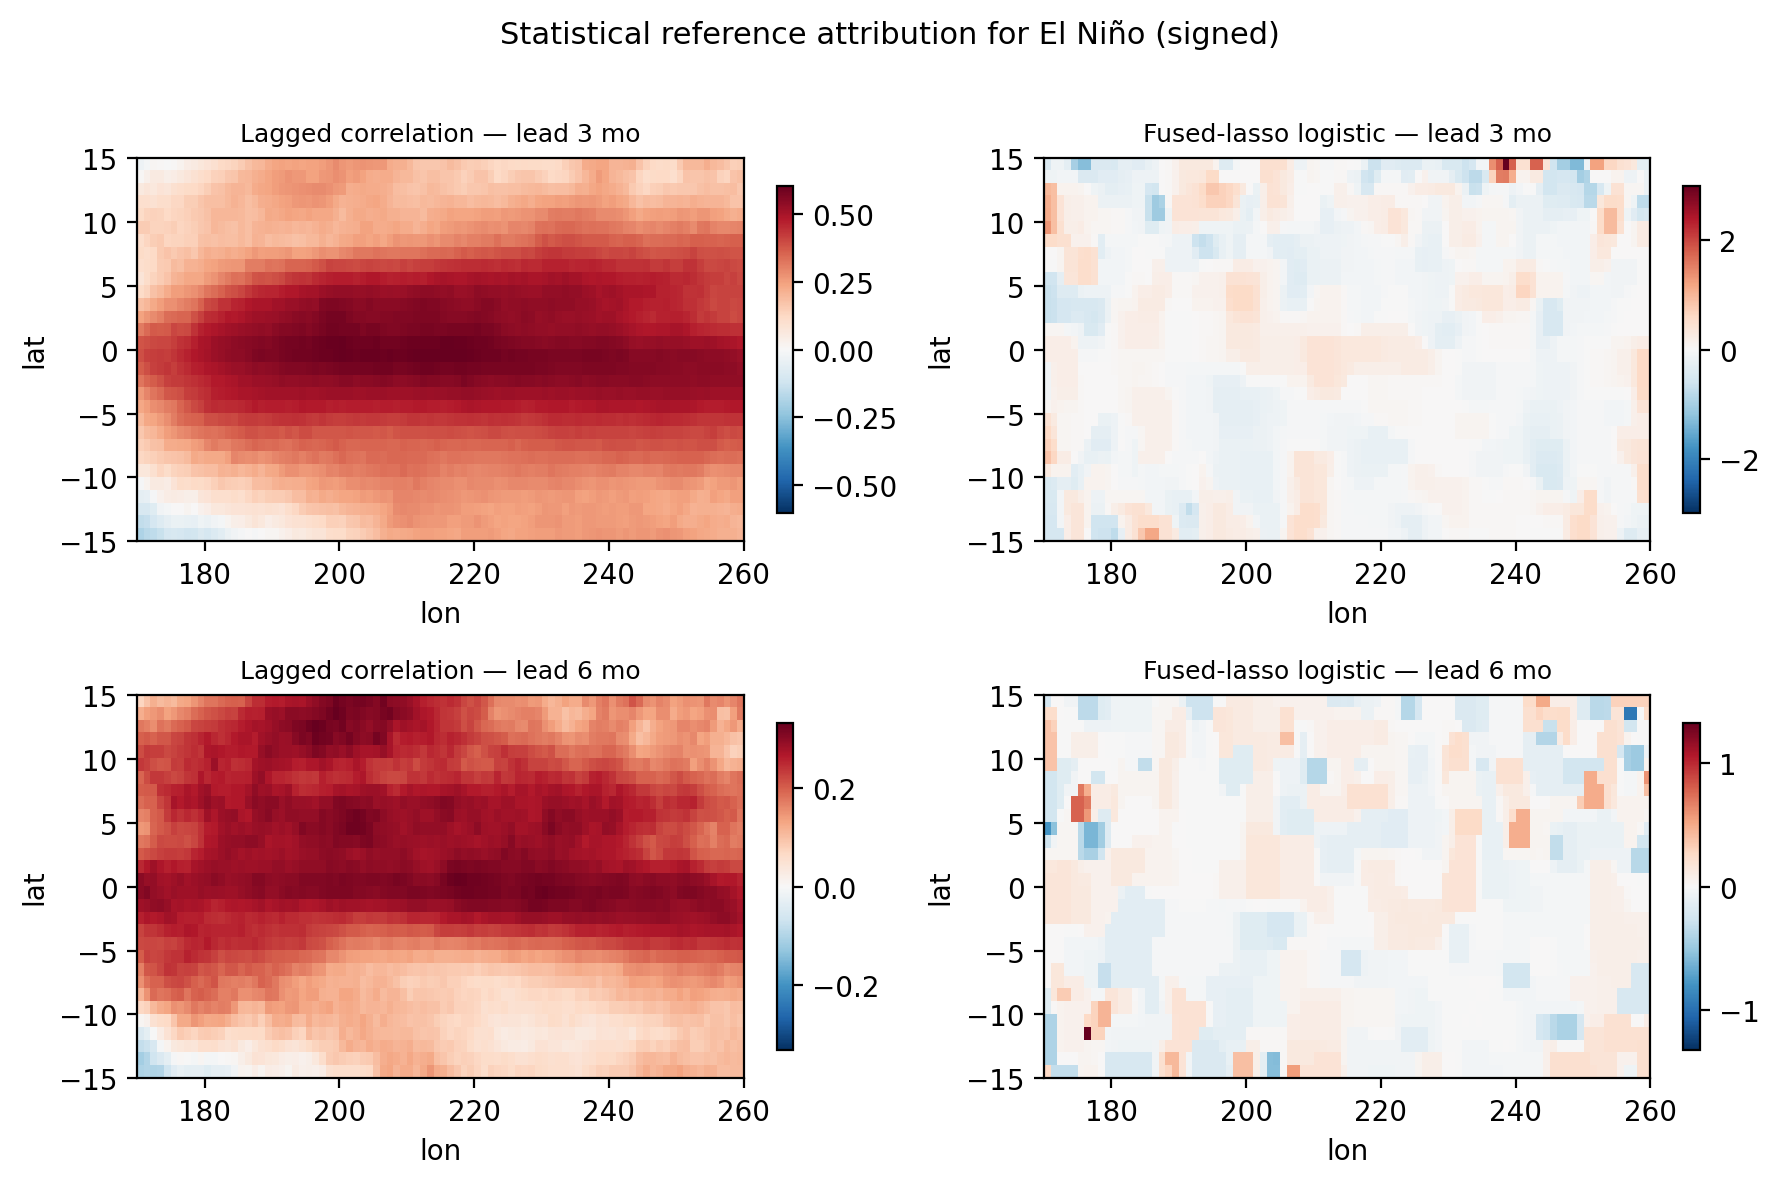
\includegraphics[width=0.95\textwidth]{sst_statistical_reference.png}
  \caption{Statistical reference attribution for El Ni\~no (signed). The lagged-correlation map
    (left) cleanly recovers the equatorial signal; the multivariate fused-lasso logistic (right)
    is destabilized by collinearity among the highly correlated equatorial cells.}
  \label{fig:enso-ref}
\end{figure}

\subsection{Do the masks agree with the statistical signal?}
Figure~\ref{fig:enso-masks} places the learned masks beside the correlation reference, and the
final column of Table~\ref{tab:enso} quantifies agreement as the Pearson correlation between the
seed-averaged mask and the magnitude of the reference. The masks \emph{recover the equatorial
signal}. At \textbf{lead 3} agreement is strong and visually unmistakable---a compact
central-Pacific blob coinciding with the correlation band, with Pearson $0.57$--$0.63$ across gate
types. At \textbf{lead 6} agreement is moderate ($0.26$--$0.50$), the masks emphasizing an
off-equatorial region broadly consistent with the broadened reference. This is convergent
validity: with no access to ground truth, two very different estimators---a univariate statistical
map and a jointly-trained nonlinear mask---independently identify the same predictive region.

Crucially, this clean agreement emerged only once the predictor was properly sized. The
over-parameterized DeepCNN of the prior specification, which generalizes worst
(Table~\ref{tab:enso-select}), produces noisy masks with essentially zero agreement at lead 3: a
model with the freedom to fit idiosyncratic noise has no need to concentrate on the physical
signal, and its attribution is correspondingly uninformative. Faithful in-model attribution thus
presupposes a well-specified predictor---an instance of the broader principle that an explanation
is only as meaningful as the model it explains, and a concrete reason to select the predictor
honestly rather than inherit an over-sized one.

\begin{figure}[htbp]
  \centering
  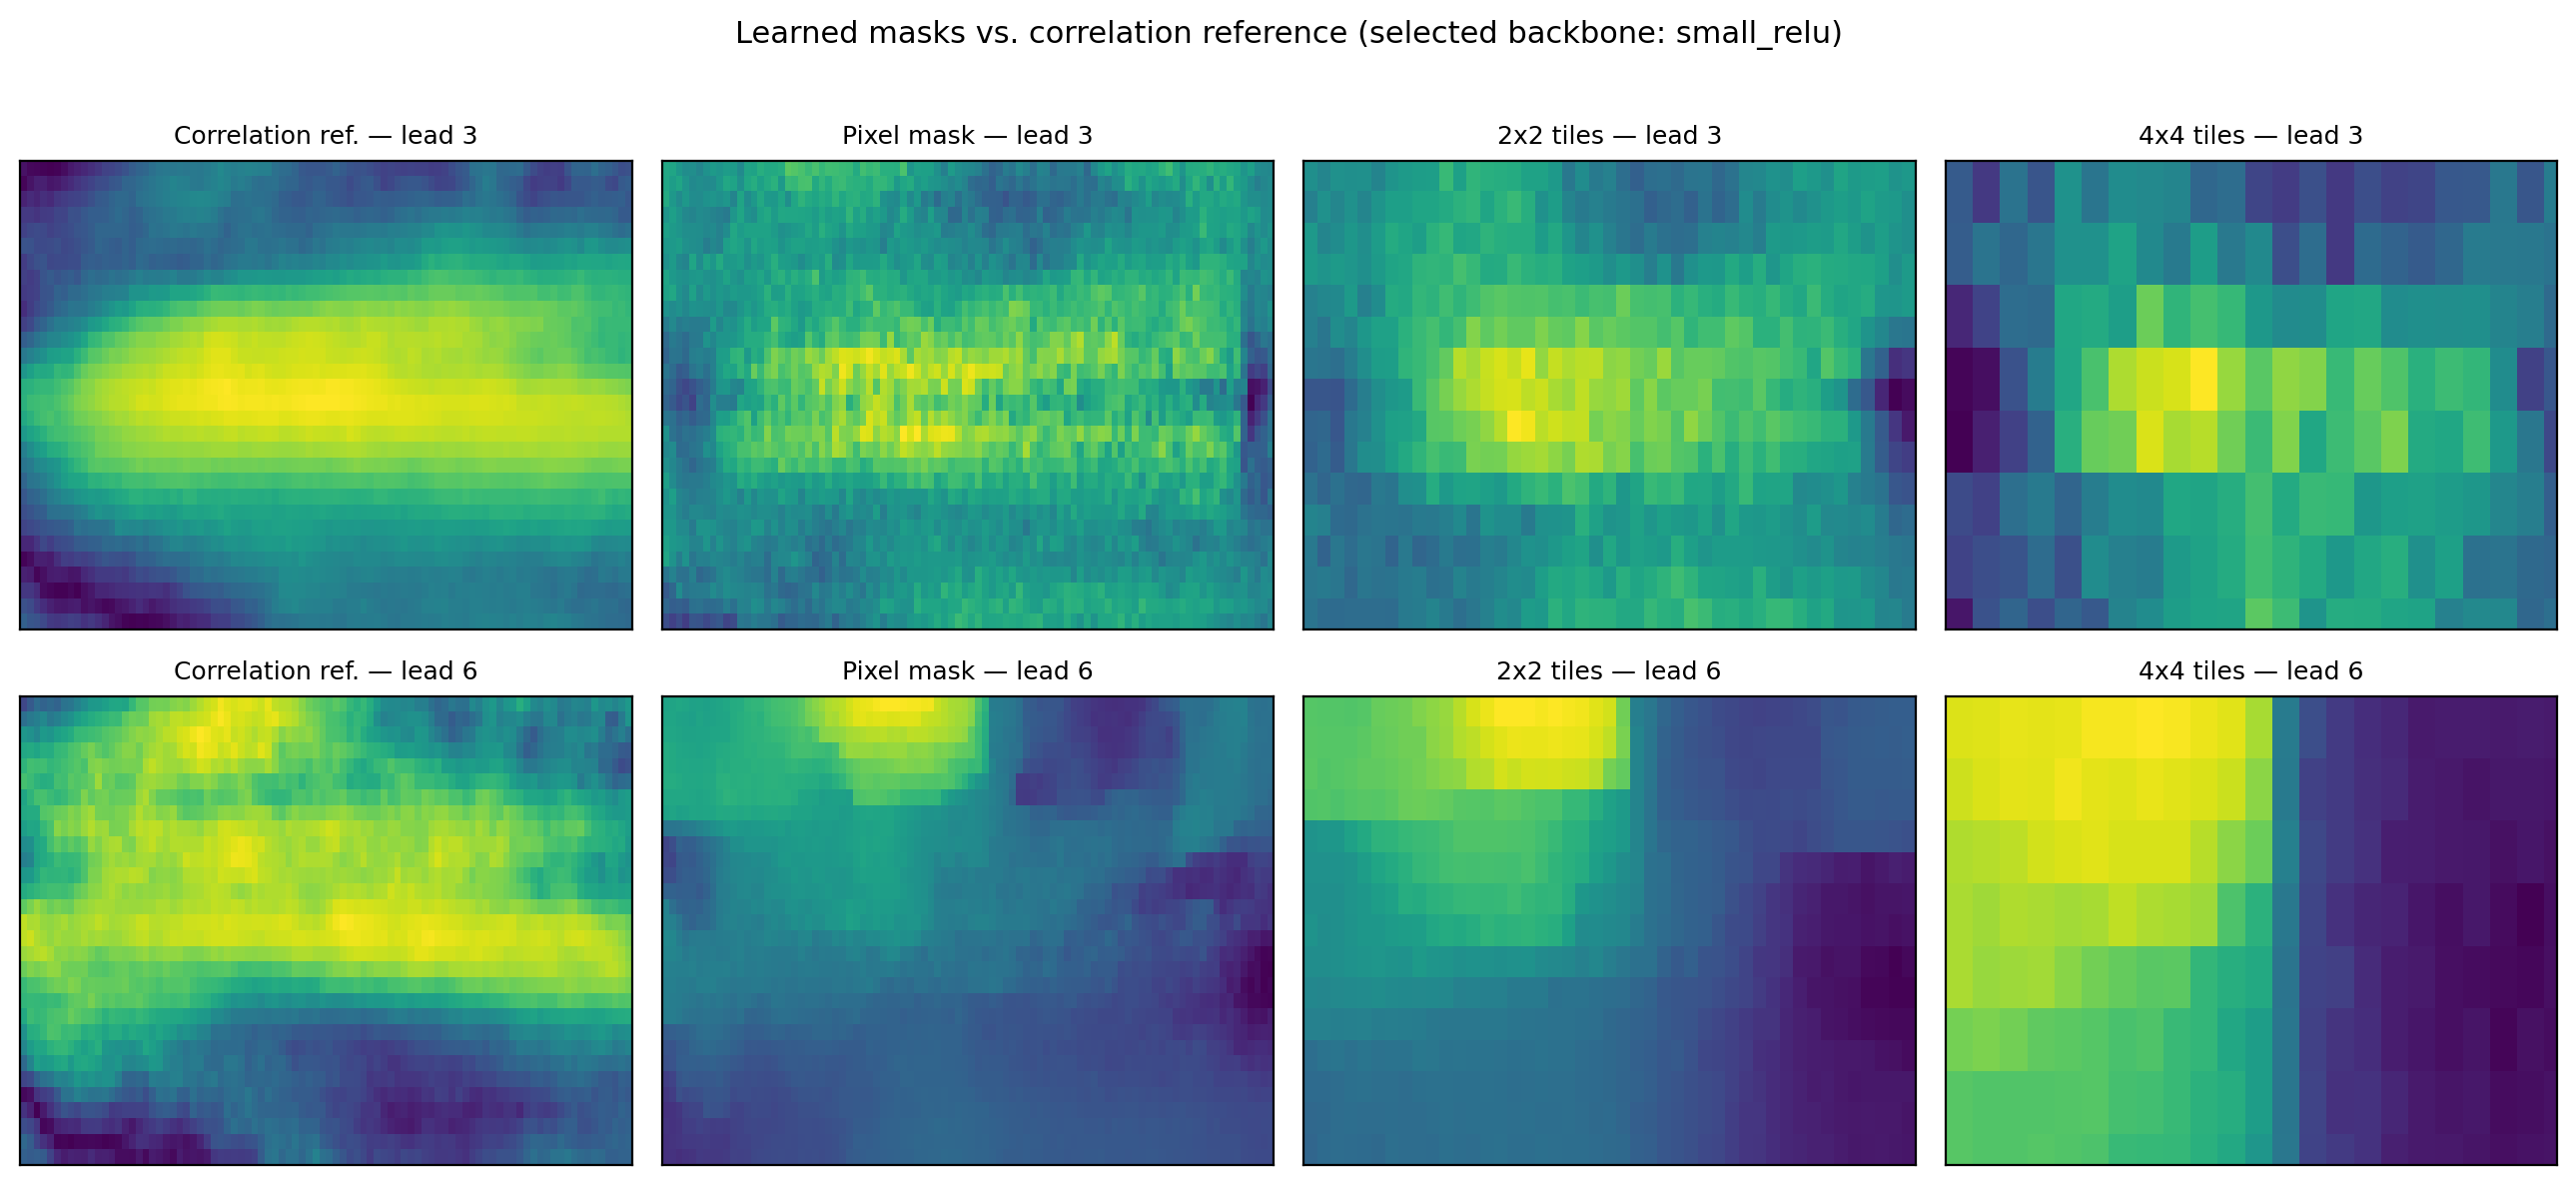
\includegraphics[width=\textwidth]{sst_masks_vs_reference.png}
  \caption{Learned input masks (pixel, $2\times2$, $4\times4$) from the selected backbone beside
    the correlation reference at leads 3 and 6. At lead 3 the masks concentrate on the equatorial
    band that the reference identifies; at lead 6 they show a consistent off-equatorial emphasis.}
  \label{fig:enso-masks}
\end{figure}

\subsection{Computational cost and the tiling knob}
The cost of the TV penalty scales with the number of mask parameters, so on the native
$0.25^\circ$ field the pixel gate is expensive ($\approx 600$\,s per fit) while tiled gates run in
seconds; on the $30\times90$ grid used above the backbone dominates and all gates train in
$\approx 23$\,s. Either way, tiling reduces the mask parameter count by a factor of $K^2$ and---as
the lead-6 agreement shows---can yield \emph{cleaner} attribution, providing a practical knob for
trading spatial resolution against computational cost in operational forecasting.

\section{Discussion}\label{sec-discussion}
Our results support two claims and expose two honest limits. On the positive side, the controlled
simulation shows that a total-variation smoothness prior \emph{measurably and significantly
improves the faithfulness} of learned in-model attribution, and does so not only for our sigmoid
mask but, applied as a modular term, for $L_0$ and stochastic-gate baselines as well---total
variation behaves as a general-purpose structured-sparsity prior for spatial attribution. Second,
among learned gates our TV+sparsity mask occupies a favourable point on the
faithfulness--accuracy frontier: it delivers faithful, spatially coherent attribution while
preserving (indeed slightly improving) predictive performance, whereas sparsity-only gates buy
sharper localization only by degrading the predictor they are meant to explain.

Two limitations temper these claims. First, the sparsity penalty rewards concentrating mask mass
on the \emph{cheapest} predictive region; when a non-causal feature is a cheap shortcut, the mask
can be captured by it (Section~\ref{sec:sim-limitation}). We therefore do not claim robustness to
spurious correlation, and identify characterizing this failure---when does sparsity-driven masking
resist versus succumb to shortcuts?---as important future work. Second, attribution faithfulness
depends on the predictor being well specified: an over-parameterized model that is free to fit
idiosyncratic noise yields masks that do not localize (Section~\ref{sec:enso}), so our
interpretability claims presuppose a model selected to generalize rather than an inherited,
over-sized one. On the predictive side our out-of-time skill is honest but limited---lead-6 ENSO
ranking is only marginally above chance---and the threshold-dependent metrics are sensitive to
temporal distribution shift. Finally, we fixed the TV weight across methods in the
modular study rather than tuning it per gate, our anomaly normalization uses the full-series
climatology (a mild, common form of leakage), and the fused-lasso reference is collinearity-limited;
each is a candidate for refinement.

Natural extensions include an uncertainty-aware variant that infers a posterior over the mask
rather than a point estimate, connecting the structured-sparsity prior used here to the
hierarchical Bayesian spatiotemporal tradition \citep{wikle2023statistical, zammit2020deep}, and a
temporal (three-dimensional) gate for spatiotemporal rather than purely spatial attribution.

\section{Conclusion}\label{sec-conclusion}
We studied total-variation--regularized input masking as a route to faithful spatial attribution
under spatial dependence. Framing the mask penalty as a structured-sparsity prior---linking total
variation, the fused lasso, and Markov-random-field smoothness to a jointly-trained attribution
gate---we showed on synthetic ground truth that the smoothness term significantly improves
attribution faithfulness across learned gating mechanisms, and that our mask trades a negligible
amount of localization for a large gain in predictive fidelity relative to sparsity-only gates.
Applied to El Ni\~no forecasting, the masks preserve predictive skill and align with a statistical
reference where attribution is well-posed, while honestly exposing the limits of attribution when
a spatially-dependent signal is highly redundant. We hope the structured-sparsity perspective on
learned attribution proves useful for interpretable modeling of high-dimensional environmental
fields.

\section{Disclosure statement}\label{disclosure-statement}
The author declares no conflict of interest.

\section{Data Availability Statement}\label{data-availability-statement}
Code and data available at: \url{https://github.com/drbob-richardson/cnn_sst}.

%%%%%%%%%%%%%%%%%%%%%%%%%%%%%%%%%%%%%%%%%%%%%%%%%%%%%%%%%%
% SUPPLEMENTARY MATERIAL
%%%%%%%%%%%%%%%%%%%%%%%%%%%%%%%%%%%%%%%%%%%%%%%%%%%%%%%%%%

\phantomsection\label{supplementary-material}
\bigskip
\begin{center}
  {\large\bf SUPPLEMENTARY MATERIAL}
\end{center}

\begin{description}
  \item[Code repository:] Full implementation, training scripts, and experiment configs (GitHub ZIP).
  \item[Dataset files:] Preprocessed versions of the datasets used in Section~\ref{sec:sim}.
  \item[Additional figures:] Ablation and sensitivity analysis figures not in the main paper.
\end{description}

%%%%%%%%%%%%%%%%%%%%%%%%%%%%%%%%%%%%%%%%%%%%%%%%%%%%%%%%%%
% REFERENCES
%%%%%%%%%%%%%%%%%%%%%%%%%%%%%%%%%%%%%%%%%%%%%%%%%%%%%%%%%%

\bibliography{bibliography.bib}

\end{document}
